\subsection{草图第一阶段}
\subsubsection{间距确定}
取\uppercase\expandafter{\romannumeral2}轴上两齿轮轴向间距$\Delta_4=10$,取中间轴上齿轮2端面至机体内壁的距离$\Delta_5=10$。
\subsubsection{\uppercase\expandafter{\romannumeral1}轴系部件设计}
\begin{enumerate}[i]
	\item 初选轴径$d_{min}$,并根据相配联轴器的尺寸确定轴径$d_1$和长度$L_1$
	\par 对于转轴,按扭转强度初算轴径,由参考文献[2]表9.4得,C=106~118,考虑轴端弯矩比转矩小,取C= 106,则$$d_{\min}=C\sqrt[3]{\frac{P}{n}}\approx 12.86$$
	\par 由于电机输出轴直径是28,经过联轴器的选取确定\uppercase\expandafter{\romannumeral1}轴的最小轴径是20。
	
	\item 选择轴的材料
	\par 因齿轮和轴径相差不大,所以制成齿轮轴,轴的材料也是40Cr。
	
	\item 确定轴的轴向固定方式
	\par 因为齿轮减速器输出轴的跨距不大,且工作温度变化不大,故轴向固定采用两端固定方式。
	
	\item 联轴器及轴段\textcircled{1}
	\par 前面计算的$d_{min}$即为轴段\textcircled{1}的直径,又考虑轴段\textcircled{1}上安装联轴器,因此轴段\textcircled{1}的设计与联轴器的设计同时进行。
	\par 由前面设计可知,选用弹性柱销联轴器。	
	\par 由参考文献\cite{1}表13.1查询可得GB/T 5014-2003中的LX2型弹性柱销联轴器符合要求,其参数为:公称转矩560$\mathrm{N}\cdot \mathrm{m}$,许用转速为6300,轴孔直径范围是$20\sim 35$。满足电动机轴径要求。取与电动机轴相连端轴径28,轴孔长度62,J型轴孔,选用A型键,联轴器主动端代号为LX2~28×62~GB/T~5014。
	\par 相应的,轴段\textcircled{1}的直径$d_1=20$,轴段长度应该比联轴器略短,故取其长度为$l_1=61$
	
	\item 密封圈与轴段\textcircled{2}
	\par 联轴器右端采用轴肩固定,取轴肩高度$h=2.45\sim 3.5$,相应的轴段②的直径范围为$24.9\sim 27$,查机械设计手册,选用轴径为25的唇型圈油封中,则轴段②的直径$d_2=25$。
	
	\item 轴承与轴段\textcircled{2}及轴段\textcircled{6}
	\par 由前面设计知,轴承类型为深沟球轴承,暂取轴承型号为6205,由参考文献\cite{1}表12.1查得内径$d=25$,外径$D=52$,宽度$B=15$,故轴段\textcircled{2}的直径$d_2=25$。
	轴段\textcircled{6}的直径应与轴段\textcircled{2}相同,即$d_6=25$。
	
	\item 轴段\textcircled{3}及轴段\textcircled{5}
	\par 取过渡轴段$d_3=d_5=27$。
	
	\item 机体与轴段\textcircled{2}\textcircled{3}\textcircled{5}\textcircled{6}的长度
	\par 因采用凸缘式轴承盖,其凸缘厚度$e=8$。由于所选联轴器不影响轴承端盖螺栓的拆卸,轴肩与轴承端盖之间的间隙取$K=18$。
	\par 在确定齿轮、机体、轴承、轴承盖的相互位置与尺寸之后,即可确定各轴段的长度。
	轴段\textcircled{2}\textcircled{6}的长度 $l_2=75$,$l_6=20$;
	轴段\textcircled{2}的长度$l_2=75$ ;
	轴段\textcircled{3}的长度 $l_3=78$。
	\par 轴的各部分尺寸均确定。取联轴器轮毂中间位置为力的作用点,可得跨距$A_1=42.5$,$B_1=100.5$,$C_1=98.5$。 
	\par 轴段\textcircled{4}长度为$l_4=30$,由于是齿轮轴所以认为轴径为齿轮分度圆的尺寸。
	\par 完成的结构草图如下所示:
	\begin{figure}[H]
		\begin{center}
			\caption{轴\uppercase\expandafter{\romannumeral1}的结构草图}
			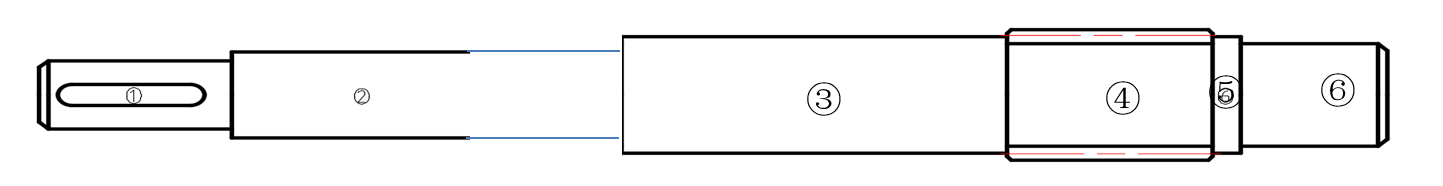
\includegraphics[width=\textwidth]{pic/zhou1.png}
		\end{center}
	\end{figure}
\end{enumerate}
\subsubsection{\uppercase\expandafter{\romannumeral2}轴轴系部件设计}
\begin{enumerate}[i]
	\item 选择轴的材料
	\par 因传递功率不大,且对质量与结构尺寸无特殊要求,故选用45钢并进行调质处理。

	\item 初选轴径$d_{min}$,并根据相配联轴器的尺寸确定轴径$d_1$和长度$L_1$
	\par 对于转轴,按扭转强度初算轴径,由参考文献[2]表9.4得,C=106~118,考虑轴端弯矩比转矩小,取C= 106,则$$d_{\min}=C\sqrt[3]{\frac{P}{n}}\approx 21.48$$
	\par 考虑键槽影响,将计算值加大5\%,取$d_{\min}=25$。
	
	\item 确定轴的轴向固定方式
	\par 因为齿轮减速器输出轴的跨距不大,且工作温度变化不大,故轴向固定采用两端固定方式。
	
	\item 	轴承与轴段\textcircled{1}及轴段\textcircled{5}
	\par 由前面设计知,轴承类型为深沟球轴承,取轴承型号为6205,由参考文献\cite{1}表12.4表12.1查得内径$d=25$,外径$D=52$,宽度$B=15$,故轴段\textcircled{1}的直径$d1=25$。
	\par 轴段\textcircled{5}的直径应与轴段\textcircled{1}相同,即$d_5=25$。

	\item 齿轮c与轴段\textcircled{2}
	\par 为了便于齿轮的安装,$d_2$应略大于$d_1$,取$d_2=30$ ,齿轮c左端用套筒固定,则轴段\textcircled{2}的长度应略小于齿轮3的宽度$b_c$,取$l_2=58$。
	
	\item 轴段\textcircled{3}
	\par 齿轮c右端用轴肩固定,轴肩高度$h=2.45\sim 3.5$,取相应的轴段\textcircled{3}的直径范围为$38.9\sim 41$,故$d_3=36$。 
	
	\item 齿轮b与轴段\textcircled{4}
	\par 齿轮b左端也用轴肩固定。可取$d_4=30$,齿轮b右端用套筒固定,则轴段\textcircled{4}的长度应略小于齿轮b的宽度$b_b$,取轴段\textcircled{4}的长度$l_4=23$。
	
	\item 轴段\textcircled{1}\textcircled{5}的长度
	\par 由草图得$l_1=37$,$l_5=40$。
	\par 轴的各部分尺寸均确定。取联轴器轮毂中间位置为力的作用点,可得跨距$A_2=69$,$B_2=52.5$,$C_2=57.5$。 
	完成的结构草图如下所示:
	\begin{figure}[H]
		\begin{center}
			\caption{轴\uppercase\expandafter{\romannumeral2}的结构草图}
			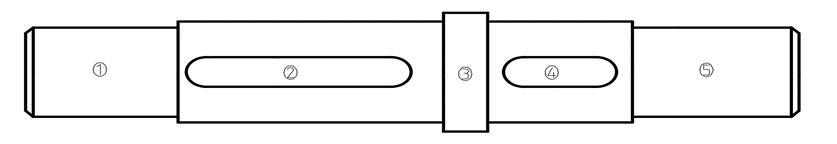
\includegraphics[width=\textwidth]{pic/zhou2.png}
		\end{center}
	\end{figure}
	(9)	键连接设计
	齿轮b、齿轮c与轴之间采用A型普通平键连接,型号分别为:\\
	键 $8\times 20$~GB/T~1096-2003,$h=7$ ,$t=4.0$ \\
	键  $8\times 56$~GB/T~1096-2003,$h=7$ ,$t=4.0$
\end{enumerate}
\subsubsection{\uppercase\expandafter{\romannumeral3}轴轴系部件设计}
\begin{enumerate}[i]
	\item 选择轴的材料
	\par 因传递功率不大,且对质量与结构尺寸无特殊要求,故选用45钢并进行调质处理。

	\item 初选轴径$d_{min}$,并根据相配联轴器的尺寸确定轴径$d_1$和长度$L_1$
	\par 对于转轴,按扭转强度初算轴径,由参考文献[2]表9.4得,$C=106\sim 118$,考虑轴端弯矩比转矩小,取C= 106,则$$d_{\min}=C\sqrt[3]{\frac{P}{n}}\approx 31.78$$

	\item 	确定轴的轴向固定方式
	\par 因为齿轮减速器输出轴的跨距不大,且工作温度变化不大,故轴向固定采用两端固定方式。
	
	\item 联轴器及轴段\textcircled{1}
	\par 前面计算的$d_{min}$即为轴段\textcircled{1}的直径,又考虑轴段\textcircled{1}上安装联轴器,因此轴段\textcircled{1}的设计与联轴器的设计同时进行。
	\par 由前面设计可知,选凸缘联轴器。由参考文献\cite{1}表13.4查询可得GB/T~5843-2003中公称转矩500 $\mathrm{N}\cdot \mathrm{m}$的凸缘联轴器满足要求,其许用转速为8000,轴孔直径范围是$30\sim 42$。取与轴相连端轴径32,轴孔长度为$L_1=70=82$,J型轴孔。相应的,轴段\textcircled{1}的直径$d_1=32$,取其长度为$l_1=82$。
	
	\item 密封圈与轴段\textcircled{2}
	\par 联轴器右端采用轴肩固定,取轴肩高度$h=2.52\sim 3.6$。查机械设计手册,选用轴径为35的唇型密封圈,则轴段②的直径$d_2=35$。
	
	\item 轴承与轴段\textcircled{2}及轴段\textcircled{6}
	\par 由前面设计知,轴承类型为深沟球轴承,取轴承型号为6207,由参考文献\cite{1}表12.1查得内径$d=35$,外径$D=72$,宽度$B=17$。故轴段\textcircled{2}的直径$d_2=35$。
	\par 轴段\textcircled{6}的直径应与轴段③\textcircled{2}相同,即$d_6=45$。
	
	\item 轴段\textcircled{5}
	\par 为了便于齿轮的安装,$d_5$应略大于$d_6$,取$d_5=40$,齿轮c右端用套筒固定,则轴段\textcircled{5}的长度应略小于齿轮d的宽度$b_d$,取$l_5=53$。
	
	\item 轴段\textcircled{4}
	\par 齿轮d右端用轴肩固定,取轴肩高度$h=3.36\sim 4.8$,取轴段\textcircled{4}的直径$d_4=46$。
	
	\item 轴段\textcircled{3}
	\par 取过渡轴段\textcircled{3}直径$d_3=40$。
	
	\item 机体与轴段\textcircled{2}\textcircled{3}\textcircled{4}\textcircled{6}的长度
	\par 因采用凸缘式轴承盖,其凸缘厚度$e=8 $。由于所选联轴器不影响轴承端盖螺栓的拆卸,轴肩与轴承端盖之间的间隙取$K=14 $。
	\par 在确定齿轮、机体、轴承、轴承盖的相互位置与尺寸之后,即可确定各轴段的长度。
	\par 取轴段\textcircled{2}的长度$l_2=65$;
	由草图得:轴段\textcircled{6}的长度$l_6=42$;轴段\textcircled{3}的长度$l_3=53$.取轴段\textcircled{4}的长度$l_4=10$。
	\par 轴的各部分尺寸均确定。取联轴器轮毂中间位置为力的作用点,可得跨距$A_3=97.5$,$B_3=96$,$C_3=59$。 
	\par 完成的结构草图如下所示。
	\begin{figure}[H]
		\begin{center}
			\caption{轴\uppercase\expandafter{\romannumeral3}的结构草图}
			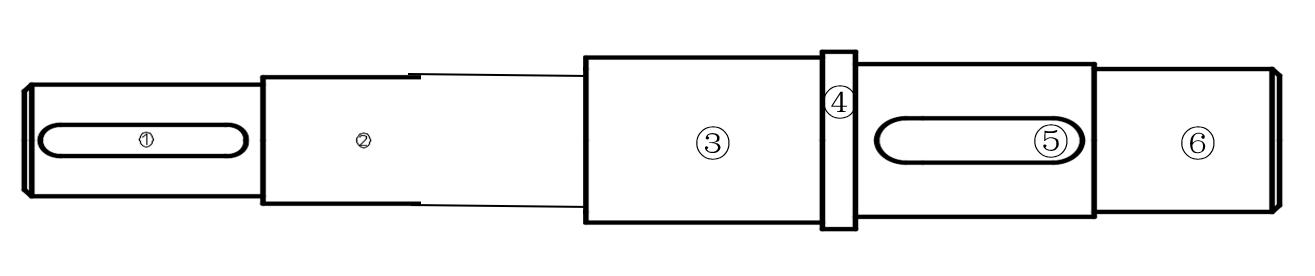
\includegraphics[width=\textwidth]{pic/zhou3.png}
		\end{center}
	\end{figure}
	\item 键连接设计
	\par 联轴器和齿轮d与轴之间采用A型普通平键连接,型号分别为:\\
	键 $10\times 80$~GB/T~1096-2003,$h=8$ ,$t=5.0$ \\
	键  $12\times 50$~GB/T~1096-2003,$h=8$ ,$t=5.0$ 
	
\end{enumerate}

\subsubsection{轴系部件校核计算}
\begin{enumerate}[i]
	\item 对\uppercase\expandafter{\romannumeral1}轴的校核
	\begin{enumerate}[A]
	\item 轴的受力分析
	\begin{enumerate}[a]
		\item 画受力简图
		\par 圆周力 $$F_t=\frac{2T_{\mathrm{{\uppercase\expandafter{\romannumeral1}}}}}{d}=1215.44$$
		径向力 $$F_r=F_t\tan{20^{\circ}}=442.38$$
		\item 计算支反力 
		\begin{figure}[H]
			\begin{center}
				\caption{轴\uppercase\expandafter{\romannumeral1}的支反力图}
				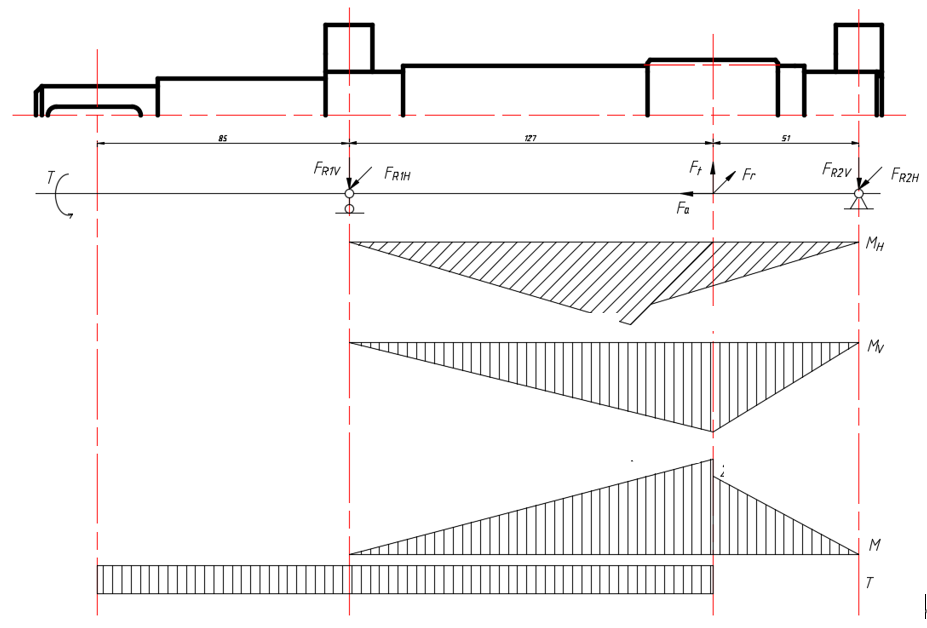
\includegraphics[width=\textwidth]{pic/jiaohe1.png}
			\end{center}
		\end{figure}
		\par 在水平面上:
		$$F_{R1H}=\dfrac{F_r\cdot C_1+F_a\cdot \dfrac{d}{2}}{B_1+C_1}=218.97$$
		$$F_{R2H}=F_r-F_{R1H}=223.41$$
		\par 在垂直平面上:
		$$F_{R1V}=\dfrac{F_t\cdot C_1}{B_1+C_1}=601.61$$
		$$F_{R2V}=F_t-F_{R1V}=613.83$$
		轴承1的总的支反力为
		$$F_{R1}=\sqrt{{F_{R1H}}^2+{F_{R1V}}^2}=640.22$$
		轴承2的总的支反力为
		$$F_{R2}=\sqrt{{F_{R2H}}^2+{F_{R2V}}^2}=653.22$$
		\item 画弯矩图
		\par 在水平面上 \\
		a-a剖面线左侧\\
		$$M_{aH}=F_{R1H}B_1=22006.49$$
		a-a剖面右侧 \\
		$$M^{\prime}_{aH}=F_{R2H}C_1=22005.89$$
		垂直面上,弯矩为\\
		$$M_{aH}=F_{R1V}B_1=60461.81$$
		合成弯矩\\
		a-a剖面左侧\\
		$$M_a=\sqrt{{M_{aH}}^2+{M_{aV}}^2}=64342.18$$
		a-a剖面右侧\\
		$$M^{\prime}_a=\sqrt{{M^{\prime}_{aH}}^2+{M_{aV}}^2}=64341.97$$
		
		\item 画转矩图$$T=1.704\times 10^4$$
	\end{enumerate}
	\item 校核轴的强度
	\par a-a剖面左侧的弯曲强度大,有转矩,为危险截面。
	\par 该截面抗弯模量为
	$$W=0.1{d_5}^3-\dfrac{bt\left(d_5-t\right)^2}{2d_5}=2667.7$$
	该截面的抗扭截面模量为
	$$W_T=0.2{d_5}^3-\dfrac{bt\left(d_5-t\right)^2}{2d_5}=5335$$
	弯曲应力$$\sigma_b=\dfrac{M}{W}=24.12$$
	$$\sigma_a=\sigma_b=24.12$$
	$$\sigma_m=0$$
	扭剪应力
	$$\tau_T=\dfrac{T}{W_T}=3.194$$
	$$\tau_a=\tau_m=\dfrac{\tau_T}{2}=1.60$$
	\par 调质处理的45钢,由参考文献\cite{2}表9.3可以查得$\sigma_b=650$,$\sigma_{-1}=300$,$\tau_{-1}=155$;材料等效系数$\psi_\sigma=0.2$,$\psi_\tau=0.1$。
	\par 因为是齿轮轴无键槽,取$K_\sigma=1$,$K_\tau=1$。
	\par 查参考文献\cite{2}表9.12得$\epsilon_\sigma=0.88$,$\epsilon_\tau=0.81$。
	\par 查参考文献\cite{2}表9.9得$\beta=1$。
	\par 由此,安全系数计算如下:
	$$S_\sigma=\dfrac{\sigma_{-1}}{\dfrac{K_\sigma}{\beta \epsilon_\sigma}\sigma_a+\psi_\sigma \sigma_m}=10.94$$
	$$S_\tau=\dfrac{\tau_{-1}}{\dfrac{K_\tau}{\beta \epsilon_\tau}\tau_a+\psi_\tau \tau_m}=72.59$$
	$$S=\dfrac{S_\sigma\cdot S_\tau}{\sqrt{{S_\sigma}^2+{S_\tau}^2}}=10.82$$
	\par 由参考文献\cite{2}表9.13得许用安全系数$\left[S\right]=1.3\sim 1.5$,显然$S>\left[S\right]$,故a-a截面安全。
	
	\item 校核键连接的强度
	\par 键连接的挤压应力\\$$\sigma_p=\dfrac{4T}{dhl}$$
	式中:d——键连接处的轴径,mm;\\
	T——传递的转矩,$\mathrm{N}\cdot \mathrm{mm}$;\\
	h——键的高度,mm;\\
	l——键连接长度,mm;
	\par 故联轴器处键连接的挤压应力为$$\sigma_p=\dfrac{4T}{dhl}=13.71$$
	\par 键、轴材料均为45钢,$\left[\sigma_p\right]= 120~150$。$\sigma_p<\left[\sigma_p\right]$,故强度满足需要。
	\item 校核轴承强度
	\par 由参考文献\cite{1}表12.4查得6205轴承的$C_r=14000$,$C_0=7880$。
	\begin{enumerate}[a]
		\item 计算轴承的轴向力
		\par 由于是深沟球轴承和圆柱齿轮,所以轴向力不予考虑。所以需要同时校核轴承1和2。
		\item 计算当量动载荷
		\par 由于是深沟球轴承和圆柱齿轮,所以无需计算当量动载荷,只需计算轴承寿命。
		\item 校核轴承寿命
		\begin{itemize}
			\item 校核轴承1的寿命
			\par 轴承在\SI{100}{\degreeCelsius}下工作,$f_T=1$。根据其载荷性质,取$f_F=1.2$。又由于是深沟球轴承、直齿轮,故$F_1=F_{R1}$,$F_2=F_{R2}$。
			\par 轴承寿命为
			$$L_h=\dfrac{10^6}{60n_{\mathrm{\uppercase\expandafter{\romannumeral1}}}}{\left(\dfrac{f_tC_r}{f_FF_{R1}}\right)}^3=71025.30$$
			\par 已知减速器使用年限为五年两班工作制,则预期寿命为
			$${L_h}^{\prime}=8\times 2\times 250\times 5=20000$$
			故轴承的寿命很充裕
			\item 校核轴承2的寿命
			\par 轴承在\SI{100}{\degreeCelsius}下工作,$f_T=1$。根据其载荷性质,取$f_F=1.2$。
			\par 轴承寿命为
			$$L_h=\dfrac{10^6}{60n_{\mathrm{\uppercase\expandafter{\romannumeral1}}}}{\left(\dfrac{f_tC_r}{f_FF_{R2}}\right)}^3=66868.62$$
			\par 已知减速器使用年限为五年两班工作制,则预期寿命为
			$${L_h}^{\prime}=8\times 2\times 250\times 5=20000$$
			故轴承的寿命很充裕
		\end{itemize}
	\end{enumerate}
\end{enumerate}	
	\item 对\uppercase\expandafter{\romannumeral3}轴的校核
	\begin{enumerate}[A]
	\item 轴的受力分析
	\begin{enumerate}[a]
		\item 画受力简图
		\par 圆周力 $$F_t=\frac{2T_{\mathrm{{\uppercase\expandafter{\romannumeral1}}}}}{d}=2598.99$$
		径向力 $$F_r=F_t\tan{20^{\circ}}=945.95$$
		\item 计算支反力 
		\begin{figure}[H]
			\begin{center}
				\caption{轴\uppercase\expandafter{\romannumeral3}的支反力图}
				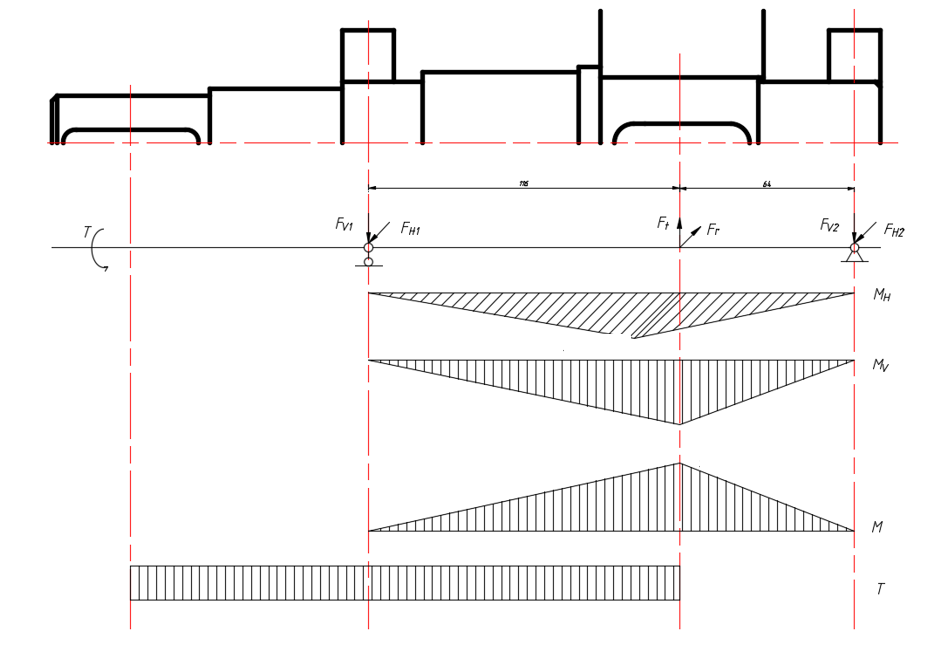
\includegraphics[width=\textwidth]{pic/jiaohe3.png}
			\end{center}
		\end{figure}
		\par 在水平面上:
		$$F_{R1H}=\dfrac{F_r\cdot C_3+F_a\cdot \dfrac{d}{2}}{B_3+C_3}=360.07$$
		$$F_{R2H}=F_r-F_{R1H}=223.41$$
		\par 在垂直平面上:
		$$F_{R1V}=\dfrac{F_t\cdot C_3}{B_3+C_3}=989.29$$
		$$F_{R2V}=F_t-F_{R1V}=1609.70$$
		轴承1的总的支反力为
		$$F_{R1}=\sqrt{{F_{R1H}}^2+{F_{R1V}}^2}=1052.88$$
		轴承2的总的支反力为
		$$F_{R2}=\sqrt{{F_{R2H}}^2+{F_{R2V}}^2}=1713.01$$
		\item 画弯矩图
		\par 在水平面上 
		$$M_{aH}=F_{R1H}B_3=34566.72$$
		垂直面上,弯矩为\\
		$$M_{aH}=F_{R1V}B_3=94971.84$$
		合成弯矩
		$$M_a=\sqrt{{M_{aH}}^2+{M_{aV}}^2}=101066.85$$
		
		\item 画转矩图$$T=2.573\times 10^5$$
	\end{enumerate}
	\item 校核轴的强度
	\par a-a剖面左侧的弯曲强度大,有转矩,为危险截面。
	\par 该截面抗弯模量为
	$$W=0.1{d_5}^3-\dfrac{bt\left(d_5-t\right)^2}{2d_5}=9610.44$$
	该截面的抗扭截面模量为
	$$W_T=0.2{d_5}^3-\dfrac{bt\left(d_5-t\right)^2}{2d_5}=20669.64$$
	弯曲应力$$\sigma_b=\dfrac{M}{W}=10.52$$
	$$\sigma_a=\sigma_b=10.52$$
	$$\sigma_m=0$$
	扭剪应力
	$$\tau_T=\dfrac{T}{W_T}=12.45$$
	$$\tau_a=\tau_m=\dfrac{\tau_T}{2}=6.22$$
	\par 调质处理的45钢,由参考文献\cite{2}表9.3可以查得$\sigma_b=650$,$\sigma_{-1}=300$,$\tau_{-1}=155$;材料等效系数$\psi_\sigma=0.2$,$\psi_\tau=0.1$。
	\par 键槽引起的应力集中系数可由参考文献\cite{2}附表9.11得:$K_\sigma=1.83$,$K_\tau=1.63$。
	\par 查参考文献\cite{2}表9.12得$\epsilon_\sigma=0.84$,$\epsilon_\tau=0.78$。
	\par 查参考文献\cite{2}表9.9得$\beta=1$。
	\par 由此,安全系数计算如下:
	$$S_\sigma=\dfrac{\sigma_{-1}}{\dfrac{K_\sigma}{\beta \epsilon_\sigma}\sigma_a+\psi_\sigma \sigma_m}=13.09$$
	$$S_\tau=\dfrac{\tau_{-1}}{\dfrac{K_\tau}{\beta \epsilon_\tau}\tau_a+\psi_\tau \tau_m}=11.70$$
	$$S=\dfrac{S_\sigma\cdot S_\tau}{\sqrt{{S_\sigma}^2+{S_\tau}^2}}=8.72$$
	\par 由参考文献\cite{2}表9.13得许用安全系数$\left[S\right]=1.3\sim 1.5$,显然$S>\left[S\right]$,故a-a截面安全。
	
	\item 校核键连接的强度
	\par 键连接的挤压应力\\$$\sigma_p=\dfrac{4T}{dhl}$$
	式中:d——键连接处的轴径,mm;\\
	T——传递的转矩,$\mathrm{N}\cdot \mathrm{mm}$;\\
	h——键的高度,mm;\\
	l——键连接长度,mm;
	\par 故联轴器处键连接的挤压应力为$$\sigma_p=\dfrac{4T}{dhl}=89.29$$齿轮处键连接的挤压应力为$$\sigma_p=\dfrac{4T}{dhl}=64.30$$
	\par 键、轴材料均为45钢,$\left[\sigma_p\right]= 120~150$。$\sigma_p<\left[\sigma_p\right]$,故强度满足需要。
	\item 校核轴承强度
	\par 由参考文献\cite{1}表12.4查得6205轴承的$C_r=14000$,$C_0=7880$。
	\begin{enumerate}[a]
		\item 计算轴承的轴向力
		\par 由于是深沟球轴承和圆柱齿轮,所以轴向力不予考虑。所以需要同时校核轴承1和2。
		\item 计算当量动载荷
		\par 由于是深沟球轴承和圆柱齿轮,所以无需计算当量动载荷,只需计算轴承寿命。
		\item 校核轴承寿命
		\begin{itemize}
			\item 校核轴承1的寿命
			\par 轴承在\SI{100}{\degreeCelsius}下工作,$f_T=1$。根据其载荷性质,取$f_F=1.2$。又由于是深沟球轴承、直齿轮,故$F_1=F_{R1}$,$F_2=F_{R2}$。
			\par 轴承寿命为
			$$L_h=\dfrac{10^6}{60n_{\mathrm{\uppercase\expandafter{\romannumeral3}}}}{\left(\dfrac{f_tC_r}{f_FF_{R1}}\right)}^3=266843.9219$$
			\par 已知减速器使用年限为五年两班工作制,则预期寿命为
			$${L_h}^{\prime}=8\times 2\times 250\times 5=20000$$
			故轴承的寿命很充裕
			\item 校核轴承2的寿命
			\par 轴承在\SI{100}{\degreeCelsius}下工作,$f_T=1$。根据其载荷性质,取$f_F=1.2$。
			\par 轴承寿命为
			$$L_h=\dfrac{10^6}{60n_{\mathrm{\uppercase\expandafter{\romannumeral3}}}}{\left(\dfrac{f_tC_r}{f_FF_{R2}}\right)}^3=61942.75$$
			\par 已知减速器使用年限为五年两班工作制,则预期寿命为
			$${L_h}^{\prime}=8\times 2\times 250\times 5=20000$$
			故轴承的寿命很充裕
		\end{itemize}
	\end{enumerate}
\end{enumerate}
	\item 对\uppercase\expandafter{\romannumeral2}轴的校核
	\begin{enumerate}[A]
	\item 轴的受力分析
	\begin{enumerate}[a]
		\item 画受力简图
		\par 圆周力 $F_{t1}=1215.44$,$F_{t2}=2598.99$ \\
		径向力 $F_{\r1}=442.38$,$F_{r2}=945.95$
		\item 计算支反力 
		\begin{figure}[H]
			\begin{center}
				\caption{轴\uppercase\expandafter{\romannumeral2}的支反力图}
				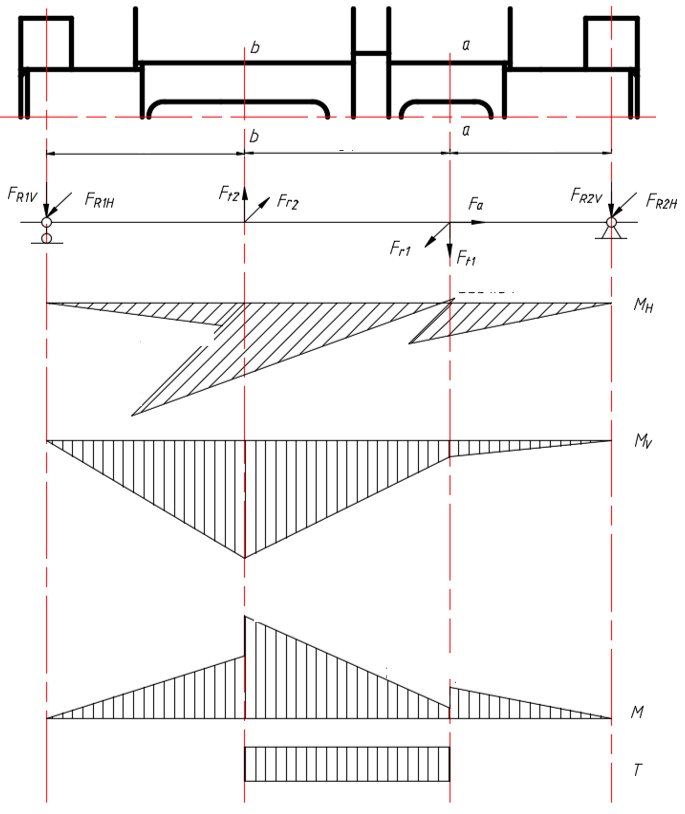
\includegraphics[width=0.8\textwidth]{pic/jiaohe2.png}
			\end{center}
		\end{figure}
		\par 在水平面上:
		$$F_{R1H}=\dfrac{F_{r2}\cdot \left(B_2+C_2\right)-F_{r1}\cdot C_2-F_a\cdot \dfrac{d}{2}}{A_2+B_2+C_2}=439.20$$
		$$F_{R2H}=F_{r2}-F_{r1}-F_{R1H}=64.37$$
		\par 在垂直平面上:
		$$F_{R1V}=\dfrac{F_{t2}\cdot \left(B_2+C_2\right)-F_{t1}\cdot C_2}{A_2+B_2+C_2}=1206.71$$
		$$F_{R2V}=F_{t2}-F_F_{t2}-F_{R1V}=176.84$$
		轴承1的总的支反力为
		$$F_{R1}=\sqrt{{F_{R1H}}^2+{F_{R1V}}^2}=1284.15$$
		轴承2的总的支反力为
		$$F_{R2}=\sqrt{{F_{R2H}}^2+{F_{R2V}}^2}=188.19$$
		\item 画弯矩图
		\par 在水平面上 \\
		a-a剖面线左侧\\
		$$M_{aH}=F_{R1H}\left(A_2+B_2\right)-F_{R2}B_2=43482.825$$
		a-a剖面右侧 \\
		$$M^{\prime}_{aH}=F_{R2H}C_2=3710.275$$
		b-b剖面线左侧\\
		$$M_{bH}=F_{R1H}A_2=30304.8$$
		b-b剖面右侧 \\
		$$M^{\prime}_{bH}=F_{R2H}\left(B_2+C_2\right)+F_{R1}B_2=77798.575$$
		垂直面上,a-a剖面
		$$M_{aV}=F_{R2V}C_2=10168.3$$
		b-b剖面
		$$M_{bV}=F_{R2V}A_2=83262.99$$
		合成弯矩\\
		a-a剖面左侧\\
		$$M_a=\sqrt{{M_{aH}}^2+{M_{aV}}^2}=44655.91$$
		a-a剖面右侧\\
		$$M^{\prime}_a=\sqrt{{M^{\prime}_{aH}}^2+{M_{aV}}^2}=10820.99$$
		b-b剖面左侧\\
		$$M_b=\sqrt{{M_{bH}}^2+{M_{bV}}^2}=88606.47$$
		b-b剖面右侧\\
		$$M^{\prime}_b=\sqrt{{M^{\prime}_{bH}}^2+{M_{bV}}^2}=113953.2526$$
		
		\item 画转矩图$$T=2.939\times 10^4$$
	\end{enumerate}
	\item 校核轴的强度
	\par b-b剖面右侧的弯曲强度大,有转矩,为危险截面。
	\par 该截面抗弯模量为
	$$W=0.1{d_2}^3-\dfrac{bt\left(d_2-t\right)^2}{2d_2}=3312,02$$
	该截面的抗扭截面模量为
	$$W_T=0.2{d_2}^3-\dfrac{bt\left(d_2-t\right)^2}{2d_2}=7342,42$$
	弯曲应力$$\sigma_b=\dfrac{M}{W}=34.41$$
	$$\sigma_a=\sigma_b=34.41$$
	$$\sigma_m=0$$
	扭剪应力
	$$\tau_T=\dfrac{T}{W_T}=4.06$$
	$$\tau_a=\tau_m=\dfrac{\tau_T}{2}=2.03$$
	\par 调质处理的45钢,由参考文献\cite{2}表9.3可以查得$\sigma_b=650$,$\sigma_{-1}=300$,$\tau_{-1}=155$;材料等效系数$\psi_\sigma=0.2$,$\psi_\tau=0.1$。
	\par 轴由两个键槽,取$K_\sigma=1.83$,$K_\tau=1.63$。
	\par 查参考文献\cite{2}表9.12得$\epsilon_\sigma=0.88$,$\epsilon_\tau=0.81$。
	\par 查参考文献\cite{2}表9.9得$\beta=1$。
	\par 由此,安全系数计算如下:
	$$S_\sigma=\dfrac{\sigma_{-1}}{\dfrac{K_\sigma}{\beta \epsilon_\sigma}\sigma_a+\psi_\sigma \sigma_m}=4.19$$
	$$S_\tau=\dfrac{\tau_{-1}}{\dfrac{K_\tau}{\beta \epsilon_\tau}\tau_a+\psi_\tau \tau_m}=36.14$$
	$$S=\dfrac{S_\sigma\cdot S_\tau}{\sqrt{{S_\sigma}^2+{S_\tau}^2}}=4.16$$
	\par 由参考文献\cite{2}表9.13得许用安全系数$\left[S\right]=1.3\sim 1.5$,显然$S>\left[S\right]$,故a-a截面安全。
	
	\item 校核键连接的强度
	\par 键连接的挤压应力\\$$\sigma_p=\dfrac{4T}{dhl}$$
	式中:d——键连接处的轴径,mm;\\
	T——传递的转矩,N·mm;\\
	h——键的高度,mm;\\
	l——键连接长度,mm;
	\par 故大齿轮处键连接的挤压应力为$$\sigma_p=\dfrac{4T}{dhl}=56.13$$小齿轮处键连接的挤压应力为$$\sigma_p=\dfrac{4T}{dhl}=21.96$$
	\par 键、轴材料均为45钢,$\left[\sigma_p\right]= 120~150$。$\sigma_p<\left[\sigma_p\right]$,故强度满足需要。
	\item 校核轴承强度
	\par 由参考文献\cite{1}表12.4查得6205轴承的$C_r=14000$,$C_0=7880$。
	\begin{enumerate}[a]
		\item 计算轴承的轴向力
		\par 由于是深沟球轴承和圆柱齿轮,所以轴向力不予考虑。所以需要同时校核轴承1和2。
		\item 计算当量动载荷
		\par 由于是深沟球轴承和圆柱齿轮,所以无需计算当量动载荷,只需计算轴承寿命。
		\item 校核轴承寿命
		\begin{itemize}
			\item 校核轴承1的寿命
			\par 轴承在\SI{100}{\degreeCelsius}下工作,$f_T=1$。根据其载荷性质,取$f_F=1.2$。
			\par 轴承寿命为
			$$L_h=\dfrac{10^6}{60n_{\mathrm{\uppercase\expandafter{\romannumeral2}}}}{\left(\dfrac{f_tC_r}{f_FF_1}\right)}^3=43126.4265$$
			\par 已知减速器使用年限为五年两班工作制,则预期寿命为
			$${L_h}^{\prime}=8\times 2\times 250\times 5=20000$$
			故轴承的寿命很充裕
			\item 校核轴承2的寿命
			\par 轴承在\SI{100}{\degreeCelsius}下工作,$f_T=1$。根据其载荷性质,取$f_F=1.2$。
			\par 轴承寿命为
			$$L_h=\dfrac{10^6}{60n_{\mathrm{\uppercase\expandafter{\romannumeral2}}}}{\left(\dfrac{f_tC_r}{f_FF_1}\right)}^3=13702541.01$$
			\par 已知减速器使用年限为五年两班工作制,则预期寿命为
			$${L_h}^{\prime}=8\times 2\times 250\times 5=20000$$
			故轴承的寿命很充裕
		\end{itemize}
	\end{enumerate}
\end{enumerate}
\end{enumerate}
